\subsection{Part Selection}
In our research for part selection we wanted to create a generalized comparison of the options we have available. We formatted this information in the tables below.

\subsubsection{Controller Subsystem}\label{sec:ps-control}
\paragraph{Minimum Requirements} At minimum, any chosen microcontrollers (MCUs) shall support natively, or by addition of a module, these features and traits:
\begin{itemize}
	\item Ability to connect to external antenna
	\item Analog-to-digital converter (ADC)
	\item IEEE 802.11
	\item In stock and available to order
	\item JTAG module or equivalent
	\item Module communication bus (UART, I2C, SPI)
	\item Network stack
	\item Onboard CPU sufficient for our purposes
	\item Onboard memory sufficient for our purposes
	\item Onboard nonvolatile memory
	\item Sockets support
	\item Pins dedicated to analog input
	\item Pins dedicated to digital I/O
\end{itemize}

\paragraph{Nice To Have} These features would be "nice to have" on any MCU selected, but are not required:
\begin{itemize}
	\item Digital-to-analog converter (DAC)
	\item Integrated antenna
	\item microSD card slot
	\item Onboard battery
	\item Pins dedicated to pulse-width modulation (PWM)
	\item Timer(s) and an RTC
	\item USB compatibility
	\item Additional wireless communication protocols (e.g. BT or BLE, Zigbee)
\end{itemize}

\paragraph{Selections} The selections, listed in \autoref{table:mcubreakdown1} and not in any particular order, match the above criteria and are being considered for selection.
\begin{table}
	\centering
	\begin{tabularx}{\textwidth}
		{
			| >{\raggedright\arraybackslash}X
			| >{\raggedright\arraybackslash}X
			| >{\raggedright\arraybackslash\columncolor[gray]{0.8}}X
			| >{\raggedright\arraybackslash}X
			| >{\raggedright\arraybackslash}X
			| >{\raggedright\arraybackslash}X
			|
		}
		\caption{MCU option breakdown}
		\label{table:mcubreakdown1} \\
		\hline
		\textbf{Model} & \textbf{\href{https://www.ti.com/tool/LAUNCHXL-CC26X2R1}{LAUNCH\-XL-CC26X2\-R1}} & \textbf{\href{https://www.ti.com/tool/LAUNCHCC3220MODASF}{LAUNCH\-CC3220\-MODASF}} & \textbf{\href{https://www.raspberrypi.com/products/raspberry-pi-pico/}{Pico W}} & \textbf{\href{https://store-usa.arduino.cc/products/arduino-nano-33-ble?selectedStore=u}{Nano 33 BLE}} & \textbf{\href{https://www.st.com/en/evaluation-tools/b-l4s5i-iot01a.html}{B-L4S5I-IOT01A}} \\
		\hline
		\textbf{Manu\-facturer} & Texas Instruments & Texas Instruments & Raspberry Pi & Arduino & STMicro\-electronics \\
		\hline
		\textbf{Micro\-controller} & CC2652R & CC3220\-MODASF & RP2040 & nRF52840 & STM32\-L4S5VIT6 \\
		\hline
		\textbf{Processor} & 1x ARM Cortex-M4F & 1x ARM Cortex-M4 & 2x ARM Cortex-M0+ & 1x ARM Cortex-M4 & 1x ARM Cortex-M4 \\
		\hline
		\textbf{Maximum Speed (MHz)} & 48 & 80 & 133 & 64 & 120 \\
		\hline
		\textbf{Memory (KB)} & 256 ROM, 352 flash, 100 SRAM & 1024 flash, 256 RAM & 16 ROM, 264 SRAM & 1024 flash, 256 SRAM & 2048 flash, 640 RAM \\
		\hline
		\textbf{Wireless capability} & BLE5.2, Zigbee, Thread & 802.11b/g/n & 802.11n & BLE5.3, Zigbee, Thread, Matter & BT4.1, 802.11b/g/n, NFC \\
		\hline
		\textbf{Serial capability} & UART, I2C, I2S, SPI & UART, I2C, SPI & UART, I2C, SPI, USB1.1 & UART, I2C, I2S, SPI, USB2.0 & UART, I2C, SPI, USB2.0 \\
		\hline
		\textbf{Price (\$)} & 40, maybe free & 60, maybe free & 6 & 28 & 53 \\
		\hline
		\textbf{ADC} & 8-channel, 12-bit & 4-channel, 12-bit & 4-channel, 12-bit & 8-channel, 12-bit & 16-channel, 12-bit \\
		\hline
		\textbf{Watchdog timer?} & No & Yes & Yes & Yes & Yes \\
		\hline
		\textbf{GPIO (pins)} & 31 & 29 & 30 & 13 & 16 \\
		\hline
		\textbf{PWM (channels)} & Supported & Supported & 16 & 4 & 6 \\
		\hline
		% \textbf{AES (bits)} & 128, 256 & 256 & Not supported & 128 & 128 \\
		% \hline
		\textbf{Required voltage (V)} & 1.8 -- 3.8 & 2.3 -- 3.6 & 1.8 -- 3.3 & 4.5 -- 21 & 4.75 -- 5.25 \\
		\hline
	\end{tabularx}
\end{table}

\paragraph{Single-board Computers} Use of single-board computers (SBCs) was considered, but will not not need to be used; sockets will be used on an MCU in conjunction with \href{https://aws.amazon.com/ec2/}{Amazon EC2} services will allow us to offload computing to a cloud solution.

\paragraph{External WiFi Module} Use of an external WiFi module is discouraged due to the following reasons:
\begin{itemize}
	\item Added cost
	\item Added complexity
	\item Modules in common use by hobbyists often have poor or no proper documentation, to the
	extent of:
	\begin{itemize}
		\item Quick start guide
		\item User's guide
		\item Datasheets
		\item Theory of operation
		\item Application uses
		\item Troubleshooting guide
		\item Schematics and mechanicals
		\item Quality and reliability
		\item Errata
	\end{itemize}
\end{itemize}
Therefore, all of the MCUs listed above support either the 802.11 or Bluetooth standards.

\paragraph{External ADC Module} Use of an external ADC was considered, and originally was decided against because an external ADC module would only add further cost and complexity to a project where the on-chip ADC is sufficiently effective for the project's requirements. The sample rate and resolution of an on-chip ADC is more than enough for our needs, and the low-cost goal of the project directly conflicts with the idea of purchasing an external ADC module.
Ultimately, the team had to use an external ADC module because the operational range of the onboard ADC was not sufficient.

\paragraph{Selection} Ultimately, the \href{https://www.ti.com/tool/LAUNCHCC3220MODASF}{LAUNCHCC3220MODASF} was chosen as the microcontroller development board for this project. In the event that the aforementioned LaunchPad is not able to be obtained, the \href{https://www.ti.com/tool/CC3220SF-LAUNCHXL}{CC3220SF-LAUNCHXL} has  quivalent capability for the project's needs.

These boards, henceforth referred to as the CC3220, are able to be requested from our university at no upfront cost to our team. This was the driving factor behind choosing the CC3220 over other microcontroller development boards. It was also determined that the microcontroller \emph{must} be able to interface via the 802.11 (WiFi) standard, for reasons that are detailed in \autoref{sec:controller_subsystem}---therefore, the LAUNCHXL-CC26X2R1 and Nano 33 BLE were disqualified from selection. The Pico W was considered due to its low cost, and the B-L4S5I-IOT01A considered because of its abundant peripherals, but both ultimately lost out to the Texas Instruments products.

\paragraph{CC3200} Due to difficulties in acquiring the CC3220 (second-generation SimpleLink device), our team made the decision to use the CC3200 (first-generation SimpleLink). These parts are mostly identical, with the differences detailed in \autoref{table:cc32x0_diff}. Development will take place on the \href{https://www.ti.com/tool/CC3200-LAUNCHXL}{CC3200-LAUNCHXL}, with the PCB MCU part to be \href{https://www.ti.com/product/CC3200}{CC3200} (if needed).

\begin{table}
	\centering
	\begin{tabularx}{\textwidth}
		{
			| >{\raggedright\arraybackslash}X
			| >{\raggedright\arraybackslash\columncolor[gray]{0.8}}X
			| >{\raggedright\arraybackslash}X
			|
		}
		\caption{Differences between CC3200 and CC3220}
		\label{table:cc32x0_diff} \\
		\hline
		\textbf{Model} & \textbf{CC3200} & \textbf{CC3220} \\
		\hline
		\textbf{Micro\-controller} & CC3200 & CC3220SF \\
		\hline
		\textbf{Secure Flash (MB)} & n/a & 1 \\
		\hline
		\textbf{Simultaneous TCP/UDP Sockets} & 8 & 16 \\
		\hline
		\textbf{WiFi Receive Sensitivity (dBm, 1 DSSS)} & -95.7 & -96 \\
		\hline
		\textbf{WiFi Receive Sensitivity (dBm, 54 OFDM)} & -74.0 & -74.5  \\
		\hline
		\textbf{Hibernate Current Draw ($\upmu$A)} & 4 & 4.5  \\
		\hline
		
	\end{tabularx}
\end{table}

\paragraph{Bill of Materials} The bill of materials for the controller subsystem can be found in \autoref{table:controller_bom}.

\begin{table}[H]
	\centering
	\begin{tabularx}{\textwidth}
		{
			| >{\raggedright\arraybackslash}l
			| >{\raggedright\arraybackslash}l
			| >{\raggedright\arraybackslash}X
			| >{\raggedright\arraybackslash}X
			| >{\raggedright\arraybackslash}X
			|
		}
		\caption{Controller subsystem bill of materials}
		\label{table:controller_bom} \\
		\hline
		\textbf{Qty} &  \begin{tabular}[c]{@{}l@{}}\textbf{Cost}\\\textbf{(\$/ea)}\end{tabular}& \textbf{Manufacturer} & \textbf{Item} & \textbf{Model Number} \\
		\hline
		1 & 0.00 & Texas Instruments & SimpleLink Wi-Fi CC3200 LaunchPad & CC3220-LAUNCHXL \\
		\hline
		2 & 10.88 & Texas Instruments & CC3200 & CC3200R1M2RGCR \\
		\hline
		2 & 3.80 & Taiyo Yuden & Surface Mount 2.4 GHz Antenna & AH316M245001-T \\
		\hline
		2 & 6.95 & Adafruit & Plastic Water Solenoid Valve & 997 \\
		\hline
	\end{tabularx}
\end{table}




% End Controller Subsystem

\subsubsection{Power Subsystem}\label{sec:ps-power}
\paragraph{Power Supply}
The power system was a key factor in this model, as we attempted to make it an independent system. This was crucial because the power system needed to be able to power all the different components while also charging itself when not operating.

As part of our goal to make the system independent, solar energy played a significant role. We needed the solar panels to operate first before powering other components. The key parts of the system included solar panels that converted light energy into electrical energy, a solar charge controller to regulate output voltage from the solar panel into the battery, and a battery to directly power the other components in the model.

We had many different sensors, electrical, and mechanical components in this model, all of which required power. To design the power system flow and operation, we first determined the total power needed for the entire system to run. This was determined by finding the individual power ratings of each component and calculating them together. Once that was done, we chose the type and quantity of battery needed for the model, taking into consideration how long we wanted the system to run, optional secondary power sources, and optional battery banks. We researched different types of solar panels, such as their efficiency and power rating. We then selected a solar charge controller, a device that sat between the solar panel and the battery to regulate how much power went into the battery. After that, we determined the voltage regulator to regulate the battery's output voltage to power the smaller components. Once we had completed all of that, we were able to find other components that would make the power system more reliable and efficient in any way.
\paragraph{Power Requirement}
Sensors, electrical, and mechanical components all required power but all consumed different amounts of power. As mentioned before, analyzing the total power requirement was important and crucial because this helped us determine the right parts that were best for this system and for the components.

With the total power determined, the Watts per hour needed for all of the components to run had to be found. The watts per hour were important too because they helped figure out how long each component would operate for. After that was found, we used the altE calculator to help pick out what kind of battery could be used, then solar panel and solar charge controller, respectively. The altE calculator was a great resource because with the proper measurements, it could help us choose what kind of battery we could use, by determining the capacity needed in watt-hours or amp-hours. This calculator could also help us choose how big of a solar panel we needed and how big of a solar charge controller we needed as well.
\paragraph{Rechargeable Battery Selection}
Solely relying on solar energy wasn’t always ideal. This was because the weather may not always guarantee sunlight, which hindered its power retention. For this reason, solar panels were paired with a battery so that the power could be stored and then used at a later time. As part of the goal to have this run as an independent system, an additional battery could be used so that one battery could power the system while the other one could charge.

There were many different types of batteries including Nickel-Cadmium, Nickel-Metal Hydride, Lithium ion, etc. Of the three batteries, they were compared to see which would best fit their model and which would fulfill the requirements on the basis of power output, efficiency, etc.

Nickel Cadmium (NiCd) batteries in today’s time were used for RC vehicles, power tools, photography equipment, and more. They were also considered as old technology. Even though they were old, they still had their advantages such as being less expensive, they were super powerful and charged fast, they required little maintenance, and more. These batteries though also had their disadvantages, one being they suffered from “ memory” problems and as a result of that, it may reduce that capacity of charges and future battery life. These batteries were also environmentally concerning because cadmium was toxic.

Nickel-Metal Hydride (NiMH) was similar to nickel cadmium, the only difference was that hydrogen was used instead of cadmium as the active element. Hybrid cars, toothbrushes, and phones were just a few of many products that used nickel-metal hydride batteries and had been used in these appliances because of the trouble-free service they granted. It was also because even being partially discharged, it could be charged as many times and would always be at full capacity. Even with advantages like that nickel-metal hydride batteries produced a lot of heat when in use, had a high self-discharge rate, and had memory issues as well, just not as bad as NiCd.

Lithium ion batteries were one of the most popular types of rechargeable batteries for portable products. They were considered the best because lithium ion batteries had high open circuit voltage, low self-discharge rates, and little to no memory effect. On top of that, they were growing within the military, electric vehicle companies, and aerospace industry with little to no maintenance. Even though they had a lot of advantages, some of the disadvantages included sensitivity towards high temperatures, it could not be fully discharged, and the cost.

Through much consideration and investigation, the four batteries listed in the following table were picked. All of which were 12V lithium iron phosphate (LiFePO4) batteries. Then the selected battery that we decided to use for the model was the Eco Worthy 12V 8Ah LiFePO4 battery. We decided to go with this battery because although it was a little expensive, the Watts per hour and the Ah rating that this battery provided, was great for what we planned on having.
\begin{table}[H]
    \centering
	
	\begin{tabularx}{\textwidth}
		{
			| >{\raggedright\arraybackslash}X
			| >{\raggedright\arraybackslash}X
			| >{\raggedright\arraybackslash}X
			| >{\raggedright\arraybackslash}X
			| >{\raggedright\arraybackslash}X
			|
		}
		\caption{Battery Selection}
		\label{table:rechargeablebatteryl} \\
		\hline
		\textbf{Manu\-facturer} & \textbf{Ampere Time} & \textbf{Eco Worthy} & \textbf{Expert\-Power} & \textbf{Eco Worthy} \\
		\hline
		\textbf{Voltage} &  12 & 12 & 12 & 12 \\
		\hline
		\textbf{mAh} &  6000 & 10000 & 5000 & 8000 \\
		\hline
		\textbf{Watt per hour} & 76.8 & 120 & 64 & 96 \\
		\hline
		\textbf{Cost} & \$29.99 & \$59.99 & \$35.99 & \$43.99 \\
		\hline
	\end{tabularx}
\end{table}
\paragraph{Solar Panel Selection}
Solar has been a growing source of energy in the past years, with new developments and breakthroughs in solar cell technology. As the whole purpose of solar energy was to collect sunlight and convert it into electrical energy, that was the minimum for this model to run as an independent system. Then, as a stretch goal, the concept of solar tracking panels was applied to create blinds with the solar panels to open and close according to the position of the sun.

On a basic level, solar panels are made of solar cells and these cells do the collecting and converting. These solar cells are made from crystalline silicon that was melted down into ingots and then cut into sheets. In the solar industry, there are 3 main types of solar panels. These types of panels were monocrystalline, polycrystalline, and thin-film panels all of which had different compositions. Each type has different efficiencies, generates different amounts of power, etc.

Monocrystalline solar panels are solar panels that are made with monocrystalline solar cells. These solar cells are composed of a single silicon crystal which provides electrons more space to move because of the electricity flow that is generated. This makes them more efficient, yet at the same time more costly. Polycrystalline solar panels are solar panels that are made with polycrystalline solar cells. Similar to monocrystalline solar cells, they are made of a silicon crystal, the only difference is that instead of a single crystal, they use several fragments of silicon to form an ingot that is cut into sheets. As a result of melting several fragments into one, this creates a mosaic look as well as giving it a blue hue, whereas the monocrystalline solar panel has a uniform color and look. Aesthetically, they may look nicer but they are less efficient than monocrystalline solar panels. This also meant that they weren’t going to be as pricey compared to the monocrystalline panels because of the efficiency and manufacturing process. Thin-film solar panels differ from crystalline solar panels greatly, all because they are made with different materials. The three main types of thin-film solar panels are amorphous silicon (a-Si), cadmium telluride (CdTe), and copper indium gallium selenide (CIGS). Currently, thin-film solar panels are the least efficient, costly, and have the shortest lifespan. It was predicted that they would have a major growth in the solar industry because although they were the least efficient, they had a higher theoretical efficiency than both monocrystalline and polycrystalline.

The choice of solar panels was based on multiple aspects of each type of solar panel. As it was known, the efficiency rating and cost from most to least went from monocrystalline, polycrystalline, and thin-film, respectively, but it was also necessary to look at its temperature coefficient, power rating, and more to be able to determine which solar panel was exactly needed. Temperature coefficient for solar panels was the power lost as the temperature rose. This played a very important role because in Florida temperatures could get hot. So, when it came to which solar panel was still more efficient in higher temperatures, monocrystalline solar panels were still the best. As follows, it then went from polycrystalline and then thin-film. It could also have been more cost-efficient as well because the other two types of solar panels were less expensive.

\begin{table}[H]
    \centering
	
	\begin{tabularx}{\textwidth}
		{
			| >{\raggedright\arraybackslash}X
			| >{\raggedright\arraybackslash}X
			| >{\raggedright\arraybackslash}X
			| >{\raggedright\arraybackslash}X
			|
		}
		\caption{Solar panel types}
		\label{table:solarpanel} \\
		\hline
		\textbf{Solar Panel Type} & \textbf{Mono\-crystalline} & \textbf{Poly\-crystalline} & \textbf{Thin - Film} \\
		\hline
		\textbf{Efficiency} &  \textgreater20\% & 15 - 17\% & 6 - 15\% \\
		\hline
		\textbf{Power Rating} &  $\le$300W & 240 - 300W & Indefinite \\
		\hline
		\textbf{Performance} & Most efficient & Efficient & Least efficient \\
		\hline
		\textbf{Temperature} & High Tolerance & Low Tolerance & High Tolerance \\
		\hline
		\textbf{Cost per Watt} & \$1 - \$1.50 & \$.70 - \$1 & \$.43 - \$.70 \\
		\hline
	\end{tabularx}
\end{table}
After conducting research and investigation, we compared different types of solar panels to determine the best fit for our model. We did not specifically choose a particular type of solar panel as all the options we considered had their benefits. However, the monocrystalline solar panel was a popular choice among the four types we evaluated. All the solar panel choices we assessed had a power rating of 10 Watts and a voltage rating of 12V, except for the Voltaic solar panel which had a voltage rating of 18V.

We ultimately selected the Eco Worthy 10W 12V monocrystalline solar panel after considering various factors. The cost of the solar panel was reasonable, and it provided excellent value for money. Its size and weight made it easy to move around, and it had received numerous positive reviews. Additionally, it was readily available for purchase on various websites.
\begin{table}[H]
    \centering
	\caption{Solar panel part breakdown}
	\label{table:solarpanelparts}
	\begin{tabularx}{\textwidth}
		{
			| >{\raggedright\arraybackslash}X
			| >{\raggedright\arraybackslash}X
			| >{\raggedright\arraybackslash\columncolor[gray]{0.8}}X
			| >{\raggedright\arraybackslash}X
			| >{\raggedright\arraybackslash}X
			|
		}
		\hline
		\textbf{Sku} & P108 & L02M10-1 & NPA10S-12H & SLP010-12U \\
		\hline
		\textbf{Manu\-facturer} & \textbf{Voltaic Systems} & \textbf{Eco Worthy} & \textbf{Newpowa} & \textbf{SolarLand} \\
		\hline
		\textbf{Solar Panel Type} & Monocrystalline & Monocrystalline & Monocrystalline & Polycrystalline \\
		\textbf{Dim\-ensions} & 10.9 x 8.8 x .16 & 13.3 x 8.1 x .7 & 14.37 x 7.68 x .91 & 14.06 x 11.89 x 1.18 \\
		\hline
		\textbf{Peak Current} & 570mA & 580mA & 630mA & 580mA \\ 
		\hline
		\textbf{Open Circuit Voltage} & 20.45V & 20.6V & 19.83V & 21.6V \\
		\hline
		\textbf{Peak Voltage} & 17.34V & 17.3V & 16.77V & 17V \\
		\hline
		\textbf{Wattage} & 9 watt & 10 watt & 10 watt & 10 watt \\
		\hline
		\textbf{Power Tolerance} & $\pm$10\% & $\pm$3\% & $\pm$3\% & $\pm$5\% \\
		\hline
		\textbf{Cost} & \$49 & \$25.99 & \$25.99 & \$35.53 \\
		\hline
	\end{tabularx}
\end{table}
\paragraph{Solar Charge Controller Selection}
Solar charge controllers played an important role in this system because the system ran on solar energy. A solar charge controller was a regulator that went in between the solar panel and the battery, regulating the total output power coming out of the solar panel. This was important because it prevented the battery from overcharging and possibly reducing its effectiveness. If the wrong charge controller had been picked, it could have resulted in a loss of power that was generated and could have harmed any device. As stated in the power requirement section, finding the total power needed for the whole system was important because it helped determine the proper charge controller to get.

There were two main types of solar charge controllers: Maximum Power Point Tracking (MPPT) and Pulse Width Modulated (PWM). Choosing the right charge controller was based on current and voltage characteristics. This was because they regulated input voltage coming in from the solar panel and output voltage of what was coming out to the battery.

Maximum power point tracking (MPPT) was a technique that observed and regulated energy coming from the solar panel and into the battery. What made this special was that it could match the solar panel voltage to the battery voltage, which allowed it to maximize the charge efficiency. They operated as a DC to DC converter, taking in high DC input from the solar panel, changing it to high AC voltage, then back down to DC voltage.

Pulse width modulated (PWM) solar charge controllers were considered the original charge controller compared to the MPPT charge controller. They were less expensive and the technique behind this controller was also simpler. On a basic level, the PWM controller acted as an on-off regulator. When the battery voltage reached a certain level, the PWM controller slowly reduced the charging current, up until the battery reached the maximum amount of energy. This made it great for smaller installations because the solar panel and the controller could match better.

While looking at different solar charge controllers, we came across 4 different controllers, all of which were PWM charge controllers. We did not specifically choose the PWM controller but through our search for what charge controller we wanted to use all of the choices we found were PWM. This was great for our model regardless because our system was not large and it was less expensive compared to MPPT charge controllers.

The solar charge controller we chose for our model was the Eco Worthy 10A PWM solar charge controller. The reason we chose this controller was because it came as a kit along with the solar panel. As a result of it coming as a kit with the solar panel, they were already very compatible together, and the price for both of them together was not expensive at all.
\begin{table}[H]
    \centering
	\begin{tabularx}{\textwidth}
			{
			| >{\raggedright\arraybackslash}X
			| >{\raggedright\arraybackslash\columncolor[gray]{0.8}}X
			| >{\raggedright\arraybackslash}X
			| >{\raggedright\arraybackslash}X
			| >{\raggedright\arraybackslash}X
			|
		}
		\caption{Charge Controller}
		\label{table:chargecontroller} \\
		\hline
		 & \textbf{LT8491} & \textbf{LTC4162} & \textbf{BQ25672} &  \textbf{BQ25713} \\
		\hline
		\textbf{Input Voltage\-Range} & 6V-80V & 4.5V-35V & 3.6V-24V & 3.5V-24V \\
		\hline
		\textbf{Charging\-Current} & 10A & 3.2A & 3A & 8.128A \\
		\hline
		\textbf{Battery\-Chemistry} & Li-Ion, Lead Acid & Lithium Phosphate/ LiFePO4 & Li-Ion/Li-Polymer, Lithium Phosphate/ LiFePO4 & Lead Acid, Li-Ion/Li-Polymer, Lithium Phosphate/ LiFePO4, NiCd, NiMH, SuperCap \\
		\hline
	\end{tabularx}
\end{table}
\begin{figure}[H]
    \caption{BQ25713 General Application Schematic}
    \centering
    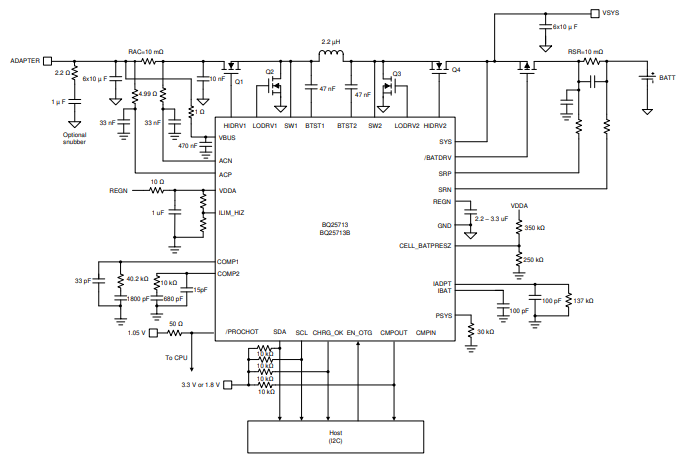
\includegraphics[width=\textwidth]{images/BQ25713_Application_Diagram.png}
    \label{fig:BQ25713 General Application Schematic}
\end{figure}
\paragraph{Voltage Regulator}
Voltage regulators played an important role in almost every electronic device. All electronic devices operated at different voltage ranges, with some requiring a constant voltage. Common operating voltages were 3V, 5V, and 12V. To provide this voltage range or constant voltage, a voltage regulator was added into the circuit design. Voltage regulators helped regulate voltages during power fluctuations and different variations in loads, preventing damage to any component. They could also regulate DC and AC voltages. For this power system, we focused on DC voltage. This was because solar panels produced DC voltage.

As previously mentioned, voltage regulators played an important role in almost every electronic device. They were used for smaller devices to power components such as sensors, op-amps, and other modules, but could also be used in bigger applications such as TVs, automotive vehicles, industrial applications, and many more. There were two main voltage regulators: linear and switching. Both of these types had the same goal, regulating a system’s voltage but operated differently depending on the application that they were used for.
\subparagraph{Linear Voltage Regulators}
Linear voltage regulators, just as the name suggests, were a type of regulator where the linear and electrical components were placed in series with the input and output. The base of the linear voltage regulator was the use of an active pass device (such as a BJT or a MOSFET) which was controlled by a high gain amplifier. To maintain a constant output voltage, the regulator used a closed feedback loop to bias the active pass device. Linear voltage regulators were also known as step-down converters because the output voltage was always less than the input voltage. As the power was consumed and dissipated in the transistor and then was converted into heat while generating a constant output voltage. In the figures below, you could see the general schematic of the linear voltage regulator but also the pin-out diagram for a LM 7805 voltage regulator. As you could see, this type of voltage regulator had three pins for input, output, and ground.
\begin{figure}[H]
    \caption{General Linear Voltage Regulator Circuit Schematic}
    \centering
    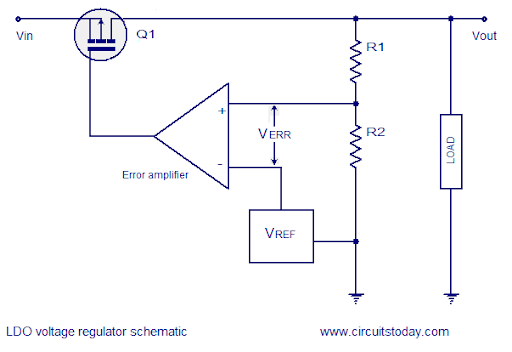
\includegraphics[width=0.5\textwidth]{images/Gen_Linear_Voltage_Regulator.png}
    \label{fig:general-linear-voltage-regulator}
\end{figure}
\begin{figure}[H]
    \caption{LM7805 Pin Diagram}
    \centering
    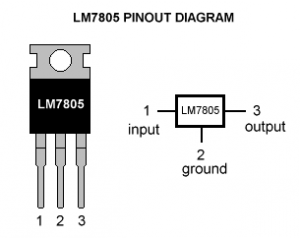
\includegraphics[width=0.5\textwidth]{images/LM7805_pin_diagram.png}
    \label{fig:LM7805-pin-diagram}
\end{figure}
Just like any electrical device, linear voltage regulators had their advantages and disadvantages. Linear voltage regulators were highly integrated devices that were simple, cheap, and responsive to changes in input voltage and load voltage. They did not produce any switching noise, which was a problem with other voltage conversion circuits. However, their biggest disadvantage was their inefficiency, which was caused by the voltage drop across the active pass device and resulted in the regulator producing a lot of heat.

Just like voltage regulators could be broken down into linear and switching voltage regulators, linear voltage regulators could be broken down into different types as well. There were two main types of linear voltage regulators: series voltage regulator and shunt voltage regulator. The main difference between the two was that with a series regulator, the active pass device was connected in series, whereas in a shunt regulator, it was connected in parallel.

As the name suggested for a series voltage regulator, the pass element in the circuit was connected in series with the load, as shown in the figure below. Looking at the circuit, the output voltage was sensed through the voltage divider network in R1 and R2, and was compared to the VREF. As a result, the voltage drop across the transistor could be varied to ensure that the voltage across the load was constant.
\begin{figure}[H]
    \caption{Series Voltage Regulator}
    \centering
    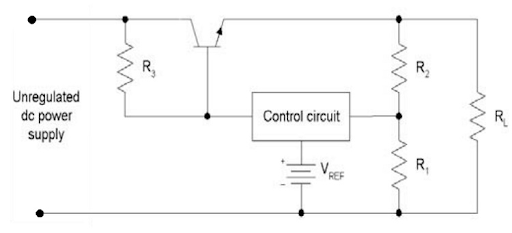
\includegraphics[width=0.5\textwidth]{images/Series_Voltage_Regulator.png}
    \label{fig:series-voltage-regulator}
\end{figure}
The main advantages of the series voltage regulator were that the current was effectively used by the load, making it more efficient than shunt voltage regulators. However, the efficiency was still low compared to a switching voltage regulator, but it was simple and the output did not have any switching spikes.

The figure below showed the circuit schematic of a shunt voltage regulator. The pass element in the circuit was connected in parallel while the resistors were connected the same as in the series voltage regulator. For this voltage regulator, voltage was maintained through the current drawn through the resistors, and as the current was varied, the output voltage across the load remained constant.
\begin{figure}[H]
    \caption{Shunt Voltage Regulator}
    \centering
    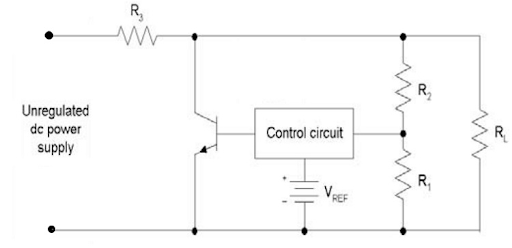
\includegraphics[width=0.5\textwidth]{images/Shunt_Voltage_Regulator.png}
    \label{fig:shunt-voltage-regulator}
\end{figure}
When compared to the series voltage regulator, it was just slightly less efficient, but was simpler to implement into the circuit. This type of linear voltage regulator was less common and was used commonly in low-powered circuits and in voltage reference circuits.
\subparagraph{Switching Voltage Regulator}
Switching voltage regulators are a type of regulator that acted as a switch, where input power was turned on until the desired voltage was reached. After the desired voltage was reached, the switch element was turned off and stopped any input power from coming in. With this type of voltage regulator, switching noise occurred because of the high-frequency from the reference voltage and the amplifier. As a result of the noise, capacitors, inductors, and other electrical components were used to smoothen out and reduce the noise. Regardless of the noise that occurred with switching voltage regulators, this type still remained very efficient because of the process of switching on and off at such high speeds. As said before, this type of regulator repeated its operation at high speeds, which allowed it to supply voltage more efficiently and reduce heat generation. The figures below show what the general schematic of a switching voltage regulator looks like but also the pin-out diagram for an lm2596 voltage regulator. You can see the difference in how many pins the lm2596 voltage regulator and the lm7805 voltage regulator have. That is because switching voltage regulators require two more pins for the switch element as well as the feedback.
\begin{figure}[H]
    \caption{General Switching Voltage Regulator}
    \centering
    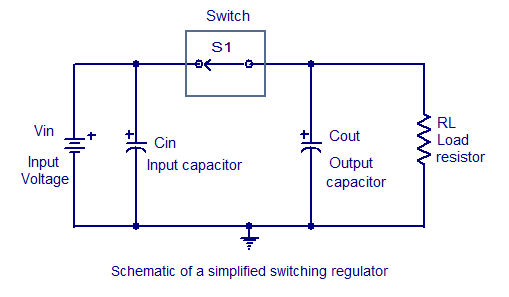
\includegraphics[width=0.5\textwidth]{images/Gen_Switching_Voltage_Regulator.png}
    \label{fig:general-switching-voltage-regulator}
\end{figure}
\begin{figure}[H]
    \caption{LM2596 Pin Diagram}
    \centering
    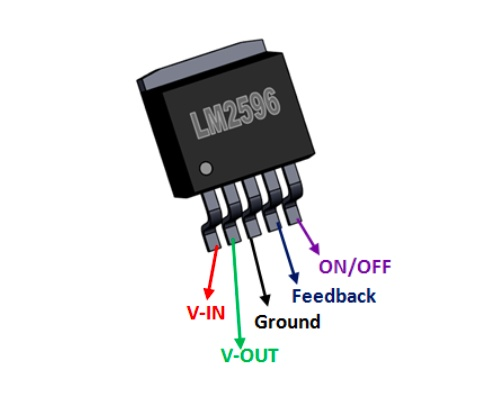
\includegraphics[width=0.5\textwidth]{images/LM2596_pin_diagram.png}
    \label{fig:lm2596-pin-diagram}
\end{figure}
Some advantages of the switching voltage regulator were that it had a much higher efficiency, did not produce a lot of heat, and was capable of higher power efficiencies. The downside was that it had a more complex design, produced more noise, which required it to have more external components added to the circuit design. The choice between linear and switching voltage regulators always depended on what it was being used for because each design required different things, but switching voltage regulators were also a popular choice because of how efficient they were with power input and their general efficiency.

There were 3 main types of switching voltage regulators: buck converter, boost converter, and buck/boost converter. These three types of voltage regulators performed similar actions but all produced different output voltages.

Buck converters, also known as step-down converters, lowered the output voltage than the input voltage. This was similar to linear voltage regulators because linear voltage regulators worked to make sure the output voltage was always lower than the input. The difference was that there was less waste. The figure below showed the circuit schematic of a buck converter. Normally, a transistor was used as the switching element, connecting and disconnecting the input voltage to the inductor.
\begin{figure}[H]
    \caption{Buck Converter (Step Down) Circuit Schematic}
    \centering
    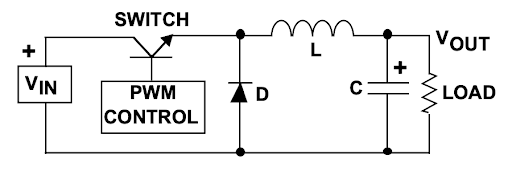
\includegraphics[width=0.5\textwidth]{images/Buck_Converter.png}
    \label{fig:buck-converter-schematic}
\end{figure}
Boost converters, also known as step-up converters, provided a higher output voltage than the input voltage. Even though the output voltage could be higher than the input voltage, the power being provided still had to be regulated within the output power specification of the circuit. Figure 8 showed the circuit schematic of the boost converter. As shown, the components were switched around compared to the buck converter. This allowed the output voltage to increase, because when the switch was on, the voltage had to go across the inductor, increasing the current. When the switch was off, the diode was forward biased and charged the load higher than the input.
\begin{figure}[H]
    \caption{Boost Converter (Step Up) Circuit Schematic}
    \centering
    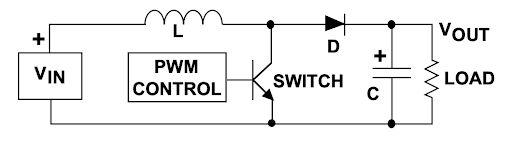
\includegraphics[width=0.5\textwidth]{images/Boost_Converter.png}
    \label{fig:boost-converter-schematic}
\end{figure}
The last type was the buck/boost converter and as the name suggests, this type of converter was able to supply either a larger or smaller output voltage, but could also invert the polarity. This type of voltage regulator was common with battery operated products because at first use the battery would supply full power but throughout time the battery as well as input power would depreciate. Figure 9 showed the circuit schematic of the buck/boost converter. This converter operated similarly to both the buck converter and the boost converter but differed because it was capable of inverting the polarity. This was done by forward-biasing the reverse-biased diode when the switch was off.
\begin{figure}[H]
    \caption{Buck/Boost Converter Circuit Schematic}
    \centering
    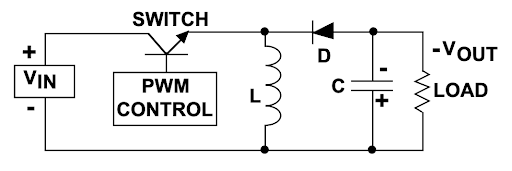
\includegraphics[width=0.5\textwidth]{images/Buck_Boost_Converter.png}
    \label{fig:buck-boost-schematic}
\end{figure}
This type of converter offered many benefits. One of the reasons it offered so much was because it brought both the buck converter and the boost converter together. It also offered lower operation cycling and was more efficient between the input and output voltages. A few downsides to this were that there was no isolation between the input and output and the output was always inverted, which resulted in complex sensing and feedback in the circuit.
\subparagraph{Voltage Regulator Selection}
The main function of a voltage regulator was to regulate output voltage from the power source, which was the 12V battery powered by solar panels, to the microcontroller and other components, ensuring that each part received the correct amount of voltage. The microcontroller we used, the Texas Instruments CC3200, operated at a 3.3V input voltage and as a result required a voltage regulator that could lower the output voltage.

As mentioned before, not all components had the same operating voltages. With the various components and voltage requirements, multiple types of voltage regulators were tested to see which one was the most efficient and best fit for our model.

For our system, we looked at the LD1117 series (Linear), LM317 (Linear), LM2576 (Switching), and LM2596 (Switching). Of the various types of regulators, these were picked because the required input voltage for the CC3200 was 3.3V. These different voltage regulators were compared based on efficiency, output voltage, cost, and any other feature that they might offer.

From the datasheets of each voltage regulator, we were able to make the comparisons in the table below.
\begin{table}[H]
    \centering
	\begin{tabularx}{\textwidth}
			{
			| >{\raggedright\arraybackslash}X
			| >{\raggedright\arraybackslash}X
			| >{\raggedright\arraybackslash}X
			| >{\raggedright\arraybackslash}X
			| >{\raggedright\arraybackslash}X
			|
		}
		\caption{Voltage Regulators}
		\label{table:voltageregulators} \\
		\hline
		\textbf{Feature} & \textbf{LD1117\-series} & \textbf{LM317} & \textbf{LM2576} &  \textbf{LM2596} \\
		\hline
		\textbf{Voltage\-Regulator Type} & Linear & Linear & Switching & Switching \\
		\hline
		\textbf{Operating Voltage} & 15V  & 3V - 40V & 3V - 40V & 4.5V - 40V \\
		\hline
		\textbf{Output Voltage} & 3.3V & 1.25V - 37V & 3.3V, 5V, 12V,\-15V & 3.3V, 5V, 12V \\
		\hline
		\textbf{Output Option} & Fixed & Adjustable & Adjustable & Adjustable \\
		\hline
		\textbf{Operating Temp} & 0$^{\circ}$C - 125$^{\circ}$C & 0$^{\circ}$C - 125$^{\circ}$C  &  -40$^{\circ}$C - 125$^{\circ}$C & -40$^{\circ}$C - 125$^{\circ}$C \\
		\hline
		\textbf{Efficiency} & $\leq$62\% & Varies & 75\% & 73\% \\ 
		\hline
		\textbf{Frequency} & N/A & N/A & 53kHz & 150kHz \\
		\hline
		\textbf{Cost (\$)} & \$0.90 & \$0.99 & \$3.69 & \$6.73 \\
		\hline
	\end{tabularx}
\end{table}
After comparing the datasheets, we agreed to select the LM317 (linear) and the LM2576 (switching). We chose these regulators so that we could further observe and compare them to determine which one would perform best and be the most suitable for our model.
\subsubsection{Sensing Subsystem}

The sensing subsystem consisted of a Visible/Near Infrared Spectrometer.

The spectrometer consisted of several optical, electrical, and mechanical components:
    \begin{itemize}
        \item Silicon Photodiode
        \item Near Infrared Spectrum InGaAs Photodiode
        \item Linear Stage Actuator Carriage Rail
        \item Reflective Diffraction Grating
        \item Focusing Lens
        \item Fiber Patch Cable      
		\item Fiber Collimator
        \item Tungsten Lamp
    \end{itemize}

\paragraph{Silicon Photodiode}
The silicon photodiode was one of the two detectors in the system, responsible for covering the visible spectrum of the soil emissions. Silicon photodiodes are cheap and overdeveloped for this application, with much of the marketing emphasizing high speed current rise times and low dark current. Our spectrometer did not require either. Instead, it was useful to have a detector with a large surface area. This reduced the precision required of other optical elements in the system while retaining the flexibility to reduce the active area of the detector with a small aperture if needed. As always, low cost was favored.
\begin{table}[H]
	\centering
	\label{table:SiliconPhotodiodes}
	\caption{Silicon Photodiodes}
	\begin{tabularx}{\textwidth}{
		|>{\raggedright\arraybackslash}X
		|>{\raggedright\arraybackslash}X
		|>{\raggedright\arraybackslash}X
		|>{\raggedright\arraybackslash}X
		|>{\raggedright\arraybackslash}X
		|>{\raggedright\arraybackslash}X
		|
	}
	\hline
	Manu-facturer & Model & Range (nm) & Area (mm\textsuperscript{2}) & Dark Current (nA) & Cost (\textdollar)\\
    \hline
	\rowcolor[gray]{.8}Newark & BPX 61 & 400-1100 & 7.02 & 2 & 13.06\\
    \hline
	Digi-key & ODD-1B & 400-1100 & 1 & 0.2 & 15.60\\
    \hline
	Digikey Opto Diode Corp & ODD-5W & 300-1100 & 5 & 1 & 14.50\\
    \hline
	Edmund Optics & PIN-3CD & 350-1100 & 3.2 & 0.15 & 34.00\\
    \hline
	Thorlabs & FD11A & 320-1100 & 1.21 & 0.002 & 15.69\\
    \hline
	Thorlabs & FDS100 & 350-1100 & 13 & 1 & 16.08\\
    \hline
	\end{tabularx}
\end{table}
The BPX 61 by Newark had a substantially better size to cost ratio than other relevant devices on the market, however it also had a higher ambient current than all others. One option was to select it and then compensate by investing in more LEDs to illuminate the target area and boost the signal up over the higher dark current, or by investing in more circuitry to clean up and boost the signal. Another option was to forgo the larger surface area and choose the sensor with the least ambient noise, Thorlabs’ FD11A. There didn’t appear to be any standout choices aside from those two. All the other devices made compromises between their specs, while these two had standout specs, but required compromises in design. The BPX 61 offered the greatest flexibility, so it was chosen for the visible-spectrum photodiode.
\paragraph{Near Infrared Spectrum InGaAs Photodiode}
The NIR InGaAs photodiode was responsible for detecting the majority of the spectral area of interest in the soil spectrometer. Once again, the relevant specs were active area, cost, and dark current. Most NIR photodetectors were designed for high-speed free space optical communication, but this application was very forgiving in terms of sensor speeds.
\begin{table}[H]
	\centering
	\label{table:InGaAsPhotodiodes}
	\caption{InGaAs Photodiodes}
	\begin{tabularx}{\textwidth}{
		|>{\raggedright\arraybackslash}X
		|>{\raggedright\arraybackslash}X
		|>{\raggedright\arraybackslash}X
		|>{\raggedright\arraybackslash}X
		|>{\raggedright\arraybackslash}X
		|>{\raggedright\arraybackslash}X
		|
	}
	\hline
	Manufacturer & Model & Range (nm) & Area (mm\textsuperscript{2}) & Dark Current (nA) & Cost (\textdollar)\\
	\hline
	Digikey Excelitas & C30617BH & 800-1700 & 0.1 & 1 & 43.58\\
	\hline
	\rowcolor[gray]{.8}Digikey Advanced Photonix & 0800-3111-011 & 800-1700 & 1.36 & 0.2 & 50.21\\
	\hline
	Thorlabs & FGA015 & 800-1700 & 0.018 & 0.5 & 63.00\\
	\hline
	Thorlabs & FGA01 & 800-1700 & 0.01 & 0.05 & 67.55\\
	\hline
	Edmund Optics & N/A & 800-1700 & 0.07 & 0.03 & 88.00\\
	\hline
	Edmund Optics & N/A & 800-1700 & 0.12 & 0.05 & 88.00\\
	\hline
	Edmund Optics & N/A & 800-1700 & 0.3 & 0.3 & 94.00\\
	\hline
	Edmund Optics & N/A & 800-1700 & 0.4 & 0.4 & 94.00\\
	\hline
	\end{tabularx}
\end{table}
The Advanced Photonix 0800-3111-011, distributed by Digikey, had the highest active area, the second lowest cost, and an acceptable midrange dark current. This made it the obvious choice for the system’s NIR detector.
\paragraph{Linear Stage Actuator Carriage Rail}
There were several methods of detecting broad spectral regimes. Scanning was much more viable than staring in this case, since staring detection required an array of detectors. This system was intended to keep costs low for the target user, and detectors were a disproportionately expensive part. Instead, this system had a pair of detectors mounted on a carriage which passed through the spatially separated beams of light. There were several important criteria for this part. It had to be able to take small, precise, increment steps in order for the detectors to capture the soil emission with high resolution. It had to have sufficient range of motion to cover the whole spectral range, from 400nm to 1700nm. And it had to meet the size, weight, and power constraints imposed by the rest of the system.
\begin{table}[H]
	\centering
	\label{table:LinearStageActuators}
	\caption{Linear Stage Actuator}
	\begin{tabularx}{\textwidth}{
		|>{\raggedright\arraybackslash}X
		|>{\raggedright\arraybackslash\columncolor[gray]{0.8}}X
		|>{\raggedright\arraybackslash}X
		|>{\raggedright\arraybackslash}X
		|>{\raggedright\arraybackslash}X
		|
	}
	\hline
	Manufacturer & Rattmmotor & TOAUTO & TOAUTO & Zeberoxyz \\
	\hline
	Model & T0601-50 & T0601-100 & T0601-101 & SFU1605 \\
	\hline
	Stroke Length (mm) & 50 & 100 & 50 & 200 \\
	\hline
	Step Angle (\textdegree) & 1.8 & 1.8 & 1.8 & 1.8 \\
	\hline
	Step Size (mm) & .005 & .005 & .005 & 0.025 \\
	\hline
	Voltage (V) & 24 & 24 & 24 & N/A \\
	\hline
	Current (A) & 0.8 & 0.6 & 0.6 & 1.6 \\
	Cost (\textdollar) & 39.00 & 67.00 & 89.00 & 83.89 \\
	\hline
	\end{tabularx}
\end{table}
The ratio between the stroke length and step size needed to be well above 1,500 in order to meet the criterion for spectral resolution. Luckily, the product with the least range was well over that limit, at 10,000:1. That allowed cost to become the driving factor. The T0601-50, distributed by Rattmmotor, was just over half the price of the next cheapest option. This was the group’s choice of scanner.
\paragraph{Reflective Diffraction Grating}
Diffraction was the operating principle behind the spectrometer. The soil emissions were composed of different wavelengths representing the chemical structure of the soil, and this was increased under illumination and then separated by diffraction. A diffraction grating separated incident electromagnetic waves of different frequencies by confining them into a tightly bounded region on reflection or transmission. This confinement caused the waves to disperse, like a prism would, with waves of higher frequencies experiencing greater dispersion. Transmission gratings were not very effective for weak signal diffraction, as in this application, because most of the optical power was concentrated straight through and not separated at all, with only weaker orders fully separating. Reflective diffraction gratings provided the best efficiency for soil spectroscopy. In order to prevent the beam from diffracting so far that it reflected straight back into itself, where it could not be collected, it was necessary to acquire a diffraction grating with grooves which were blazed at an angle, so that the surface normal of the grating had a greater angle than 90 degrees. The blaze angle corresponding to the 1000 nm diffraction regime sufficed. Next, it was necessary to calculate the angular spread of diffraction from 400nm to 1700nm off a diffraction grating from several incident angles. The first order diffraction must not overlap with the incident beam if it was to be measured. Increased size was also desirable, in order to maximize the number of wave-groove interactions and boost diffraction efficiency.
\begin{table}[H]
	\centering
	\label{table:DiffractionGratings}
	\caption{Diffraction Gratings}
	\begin{tabularx}{\textwidth}{
		|>{\raggedright\arraybackslash}X
		|>{\raggedright\arraybackslash}X
		|>{\raggedright\arraybackslash}X
		|>{\raggedright\arraybackslash}X
		|>{\raggedright\arraybackslash}X
		|>{\raggedright\arraybackslash}X
		|
	}
	\hline
	Manu\-facturer & Model & Density lines/mm & Dimensions (mm) & Blaze Angle (nm) & Cost (\textdollar)\\
	\hline
	Thorlabs & GR13-0610 & 600 & 12.7x12.7x6 & 1000 & 76.58\\
	\hline
	Thorlabs & GR25-1210 & 1200 & 25x25x6 & 1000 & 125.77\\
	\hline
	Edmund Optics & Stock 43-745 & 600 & 12.7x12.7x6 & 1000 & 80.00\\
	\hline
	Edmund Optics & Stock 43-753 & 1200 & 12.7x12.7x6 & 1000 & 80.00\\
	\hline
	MKS Newport & 33025FL01-520R & 600 & 12.5x12.5x6 & 1000 & 155.00\\
	\hline
	MKS Newport & 33025FL01-530R & 1200 & 12.5x12.5x7 & 1000 & 155.00\\
	\hline
	\rowcolor[gray]{.8}ScienceTech & 631-0024 & 1200 & 50x50x9.5mm & 1000 & 500.00\\
	\hline
	\end{tabularx}
\end{table}
The spectral regime was too wide to be able to reliably use a 600 nm grating without losing information in the infrared. Unfortunately, efficiency was not a variable that could be compared from product to product, since it varied with wavelength and per polarization. This meant the only remaining comparison was the ratio from cost to active area. ScienceTech was ruled out immediately. Its cost to size ratio was not far from the other 1200 nm gratings on this list, but it would have been difficult to justify doubling the project budget in order to achieve a marginal increase in grating power efficiency. This spec could also be compensated by cranking up the optical power probing the soil, presumably for less than the \textdollar45 difference between the Edmund Optics and Thorlabs models.
\paragraph{Focusing Optic}
The spectrometer needed a lens to focus each separated beam of unique wavelength onto a spot the size of the sensor. NBK-7 glass was a cheap, high-quality material popular for these applications, making it the obvious choice for the focusing optic. Ray tracing analysis showed that the optimal lens had a focal length of approximately 50mm and a diameter or height of 30mm or about 1 inch. The effective focal length was a soft constraint, since the position of the lens contributed to total focus. However, the diameter of the lens was a hard constraint. This was because if the lens was too wide, it would block the input beam before it hit the diffraction plate. The lens could either be biconvex spherical or cylindrical, with the advantage of plano-cylindrical lenses being that they required fewer parts to mount. In this design, while the width of the lens was a limiting factor, the center thickness and weight were unbounded.
\begin{table}[H]
	\centering
	\label{table:Focusing Optic}
	\caption{Focusing Optic}
	\bigskip
	\begin{tabular}{|p{3cm}|p{2.5cm}|p{2cm}|p{1.5cm}|p{1.75cm}|p{1.25cm}|}
	\hline
	Model & Manufacturer & Shape & Focal Length (mm) & Diameter /Height (mm) & Cost (\textdollar)\\
	\hline
	Stock \#45-163 & Edmund Optics & Spherical & 50 & 30 & 39.00\\
	\hline
	SLB-30B-50P & Opto Sigma & Spherical & 51.1 & 30 & 42.84\\
	\hline
	LB1471 & Thorlabs & Spherical & 50 & 25.4 & 26.95\\
	\hline
	Stock \#35-024 & Edmund Optics & Cylindrical & 50 & 25.4 & 67.00\\
	\hline
	LJ1695L1 & Thorlabs & Cylindrical & 50 & 32 & 126.96\\
	\hline
	\end{tabular}
\end{table}
The priority was optical focus, however, the wide selection of lens designs available ensured that this target could be reached exactly. Since lens diameter was the next limiting factor, the LB1471 and the Edmund Optics Stock \#35-024 were preferred. While the other models might have technically been small enough to avoid obstructing the input beam headed towards the diffraction grating, by going several millimeters under the maximum value, the lens position could be adjusted closer to the grating, allowing for greater flexibility of focal length. The cost of the cylindrical \#35-024 was two and a half times that of the spherical LB1471. While it might have been simpler to mount, it could not have been simple enough to justify the high cost. Our choice of lens was the LB1471.
\paragraph{Fiber Optic Patch Cable}
To transmit the Electromagnetic waves from the soil to the spectrometer, we needed a waveguide. Fiber optics were chosen as a cheap, flexible waveguide coated in a durable jacket material, and fiber patch cables came with precision optical surfaces at either end, as well as attachments for connecting to lens mounts and other optical fibers. The beam coupled into the fiber was diffuse because it was being scattered off the surface of the soil. The fiber needed to have the largest possible core diameter and numerical aperture, so it was a multimode fiber. The standard connector in spectroscopy devices was the SMA (subminiature assembly). The fiber was contained within a space of less than a cubic meter, so 2 meters were sufficient for all flexibility and attenuation per kilometer was negligible with one exception. Fiber glass with trace amounts of hydroxyl ions tended to absorb optical power at around 700nm and 950nm, which was problematic because this interfered with determining whether this material was present in the soil matrix. Low OH fibers were preferred because they minimized this absorption. Thorlabs sold a variety of fiber patch cables with Low OH and a spectral range from 400nm to 2000nm and higher.

There were a wide range of fiber patch cable producers, however the above constraints ruled out the majority of suppliers, either because they did not have documentation indicating whether the material had low Hydroxyl ion concentrations or because the fiber patch cables they offered came with unnecessary features like armor cabling or antireflective coating. Thorlabs offered the only real options for comparison.
\begin{table}[H]
	\centering
	\label{table:Fiber Optic Patch Cable}
	\caption{Fiber Optic Patch Cable}
	\bigskip
	\begin{tabular}{|p{2cm}|p{2.5cm}|p{2cm}|p{2.75cm}|p{1.75cm}|}
	\hline
	Model & Manufacturer & Numerical Aperture & Core Diameter (um) & Cost (\textdollar)\\
	\hline
	M45L02 & Thorlabs & 0.5 & 365 & 93.63\\
	\hline
	M44L02 & Thorlabs & 0.5 & 200 & 88.46\\
	\hline
	M28L02 & Thorlabs & 0.39 & 400 & 110.95\\
	\hline
	M38L02 & Thorlabs & 0.39 & 200 & 88.46\\
	\hline
	M14L02 & Thorlabs & 0.22 & 50 & 82.99\\
	\hline
	\end{tabular}
\end{table}
After all other design decisions were made, the three remaining criteria were Numerical Aperture, Core Diameter, and Cost. M14L02 was the cheapest model, but not by much, and the low Numerical aperture would have reduced the total light that could have been focused into the fiber. This could not have been fixed with additional lenses. Models M38L02 and M44L02 were the next cheapest. They boasted a much greater core diameter, and one of them had the maximum typical numerical aperture for glass fiber. The M45L02 and M28L02 had the largest core diameters, but in the M28L02 model, this came with a reduced numerical aperture, which decreased input optical power, making it inferior to the M45L02. The M45L02 and M44L02 stood out as having the maximum possible Numerical aperture. Between the two, the question was whether the extra core size was worth the 5\textdollar for added performance. This was difficult to determine theoretically, but since the greatest difficulty of the system was achieving sufficient signal to noise ratio, we erred on the side of caution and chose model M45L02, which best transmitted a clear signal.
\paragraph{Fiber Collimator}
As stated above, the beam that needed to be coupled into the fiber was not collimated by the light source, the soil, or the fiber. In order for it to be coupled into the beam, a fiber collimator was needed. Fiber optic cables came with attachments that housed lens arrays focused at the surface of the fiber core. This allowed light coming into the lens to be coupled into the fiber, and light coming out of the fiber to be collimated into a beam. Fiber collimators could be mechanical, optical, or optomechanical, depending on the application. Fixed collimating packages were the cheapest solution with compatible mounting for SMA fiber cables. Thorlabs offered three relevant models.
\begin{table}[H]
	\centering
	\label{table:Fiber Collimator}
	\caption{Fiber Collimator}
	\bigskip
	\begin{tabular}{|p{2cm}|p{2.5cm}|p{2cm}|p{2.75cm}|p{1.75cm}|}
	\hline
	Model & Manufacturer & Numerical Aperture & Output Beam Diameter (mm) & Cost (\textdollar)\\
	\hline
	F240SMA-980 & Thorlabs & 0.5 & 1.7 & 177.45\\
	\hline
	F110SMA-980 & Thorlabs & 0.37 & 1.35 & 177.45\\
	\hline
	F220SMA-980 & Thorlabs & 0.25 & 2.4 & 177.45\\
	\hline
	\end{tabular}
\end{table}


Since cost is equivalent for all models, the only factors are numerical aperture and beam size. All three beam sizes are acceptable and will not have a significant impact on the system quality. In order to maximize the amount of light that can be coupled into the fiber, the numerical aperture will be selected to match that of the fiber. Our group selected Model F240SMA-980 for these reasons.

\paragraph{Bill of Materials}
The BOM for the sensing subsystem can be found in the table below.

\begin{table}[H]
	\centering
	\label{table:SensingBOM}
	\caption{Sensing Subsystem Bill of Materials}
	\bigskip
	\begin{tabular}{|p{2cm}|p{2.5cm}|p{2cm}|p{2.75cm}|p{1.75cm}|}
	\hline
	Qty & Cost (\textdollar) & Manufacturer & Item & Model\\
	\hline
	1 & 13.06 & Newark & VIS Photodiode & BPX 61\\
	\hline
	1 & 50.21 & Excelitas & NIR Photodiode & 0800-3111-01\\
	\hline
	1 & 30.76 & Rattmmotor & Linear Rail Actuator & T0601-50\\
	\hline
	1 & 30.76 & Edmund Optics & Blazed Reflection Grating & 43-753\\
	\hline
	1 & 30.76 & Thorlabs & Biconvex Lens & LB1471\\
	\hline
	1 & 30.76 & Thorlabs & Fiber Patch Cable & M45L02\\
	\hline
	1 & 30.76 & Thorlabs & Fiber Collimator & F240SMA-980\\
	\hline
	1 & 30.76 & Osram Sylvania & Tungsten Halogen Bulb & 54262\\
	\hline
	\end{tabular}
\end{table}